% Options for packages loaded elsewhere
\PassOptionsToPackage{unicode}{hyperref}
\PassOptionsToPackage{hyphens}{url}
\documentclass[
  spanish,
]{article}
\usepackage{xcolor}
\usepackage[margin=1in]{geometry}
\usepackage{amsmath,amssymb}
\setcounter{secnumdepth}{5}
\usepackage{iftex}
\ifPDFTeX
  \usepackage[T1]{fontenc}
  \usepackage[utf8]{inputenc}
  \usepackage{textcomp} % provide euro and other symbols
\else % if luatex or xetex
  \usepackage{unicode-math} % this also loads fontspec
  \defaultfontfeatures{Scale=MatchLowercase}
  \defaultfontfeatures[\rmfamily]{Ligatures=TeX,Scale=1}
\fi
\usepackage{lmodern}
\ifPDFTeX\else
  % xetex/luatex font selection
\fi
% Use upquote if available, for straight quotes in verbatim environments
\IfFileExists{upquote.sty}{\usepackage{upquote}}{}
\IfFileExists{microtype.sty}{% use microtype if available
  \usepackage[]{microtype}
  \UseMicrotypeSet[protrusion]{basicmath} % disable protrusion for tt fonts
}{}
\makeatletter
\@ifundefined{KOMAClassName}{% if non-KOMA class
  \IfFileExists{parskip.sty}{%
    \usepackage{parskip}
  }{% else
    \setlength{\parindent}{0pt}
    \setlength{\parskip}{6pt plus 2pt minus 1pt}}
}{% if KOMA class
  \KOMAoptions{parskip=half}}
\makeatother
\usepackage{graphicx}
\makeatletter
\newsavebox\pandoc@box
\newcommand*\pandocbounded[1]{% scales image to fit in text height/width
  \sbox\pandoc@box{#1}%
  \Gscale@div\@tempa{\textheight}{\dimexpr\ht\pandoc@box+\dp\pandoc@box\relax}%
  \Gscale@div\@tempb{\linewidth}{\wd\pandoc@box}%
  \ifdim\@tempb\p@<\@tempa\p@\let\@tempa\@tempb\fi% select the smaller of both
  \ifdim\@tempa\p@<\p@\scalebox{\@tempa}{\usebox\pandoc@box}%
  \else\usebox{\pandoc@box}%
  \fi%
}
% Set default figure placement to htbp
\def\fps@figure{htbp}
\makeatother
\ifLuaTeX
\usepackage[bidi=basic]{babel}
\else
\usepackage[bidi=default]{babel}
\fi
% get rid of language-specific shorthands (see #6817):
\let\LanguageShortHands\languageshorthands
\def\languageshorthands#1{}
\setlength{\emergencystretch}{3em} % prevent overfull lines
\providecommand{\tightlist}{%
  \setlength{\itemsep}{0pt}\setlength{\parskip}{0pt}}
\usepackage{booktabs}
\usepackage{longtable}
\usepackage{array}
\usepackage{multirow}
\usepackage{float}
\usepackage{colortbl}
\usepackage{xcolor}
\usepackage{pdflscape}
\usepackage{geometry}
\geometry{margin=2.5cm}
\usepackage{fancyhdr}
\pagestyle{fancy}
\fancyhead[L]{\small Conclusiones}
\fancyhead[R]{\small Tesis --- Experiencia Gastronómica}
\fancyfoot[C]{\thepage}
\renewcommand{\headrulewidth}{0.4pt}
\usepackage{caption}
\captionsetup{font=small, labelfont=bf}
\usepackage{indentfirst}
\setlength{\parindent}{1.25cm}
\usepackage{bookmark}
\IfFileExists{xurl.sty}{\usepackage{xurl}}{} % add URL line breaks if available
\urlstyle{same}
\hypersetup{
  pdftitle={Conclusiones},
  pdfauthor={Martín Vargas Estrada},
  pdflang={es},
  hidelinks,
  pdfcreator={LaTeX via pandoc}}

\title{Conclusiones}
\usepackage{etoolbox}
\makeatletter
\providecommand{\subtitle}[1]{% add subtitle to \maketitle
  \apptocmd{\@title}{\par {\large #1 \par}}{}{}
}
\makeatother
\subtitle{Impacto de los factores de la experiencia gastronómica en la
toma de decisiones del comensal}
\author{Martín Vargas Estrada}
\date{21 de March de 2026}

\begin{document}
\maketitle

{
\setcounter{tocdepth}{3}
\tableofcontents
}
\newpage

\section{Objetivo General}\label{objetivo-general}

\begin{quote}
\emph{Determinar cómo los tres factores de la experiencia gastronómica:
calidad del producto, calidad del servicio y entorno, impactan en la
toma de decisiones del comensal.}
\end{quote}

\subsection{Conclusión General}\label{conclusiuxf3n-general}

Queda estadísticamente demostrado que la variación del nivel de calidad
para cada dimensión de la experiencia culinaria (producto, servicio y
entorno) impacta, en efecto, sobre las tres variables que constituyen la
toma de decisiones del comensal: Satisfacción, Intención de Revisitar
(ver Resultado 2.1) y Recomendar o no (ver Resultado 2.2.). Además, el
tamaño de este efecto es considerable en las tres variables
dependientes.

Por lo demás el análisis paramétrico (ANOVA de Welch) ratifica este
hallazgo, lo cual brinda solidez a esta conclusión.

\subsection{Objetivo Específico: Impacto de la Manipulación del
Producto}\label{objetivo-especuxedfico-impacto-de-la-manipulaciuxf3n-del-producto}

\begin{quote}
\emph{Identificar de qué manera los cambios en la calidad del producto
influyen en la toma de decisiones del comensal.}
\end{quote}

\subsubsection{Impacto de la Manipulación del Producto sobre la
Satisfacción}\label{impacto-de-la-manipulaciuxf3n-del-producto-sobre-la-satisfacciuxf3n}

Para detallar los resultados estadísticos del impacto específico de la
manipulación del producto sobre la Satisfacción del comensal, tenemos el
siguiente gráfico:

\begin{figure}[H]

{\centering 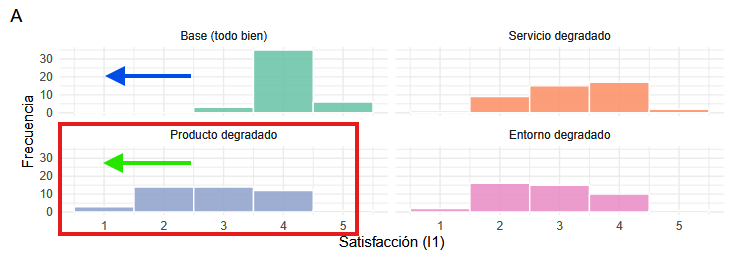
\includegraphics[width=0.7\linewidth]{Sat_P} 

}

\caption{Impacto de la Manipulación de las variables independientes sobre la Satisfacción del Comensal.}\label{fig:unnamed-chunk-1}
\end{figure}

En la Figura 1 apreciamos que a resultas de la degradación del Producto
(zona recortada en rojo) el nivel de Satisfacción se desplaza hacia la
izquierda (flecha verde, comparada con la flecha azul, que grafica la
distribución de los puntajes en la línea base).

\begin{figure}[H]

{\centering 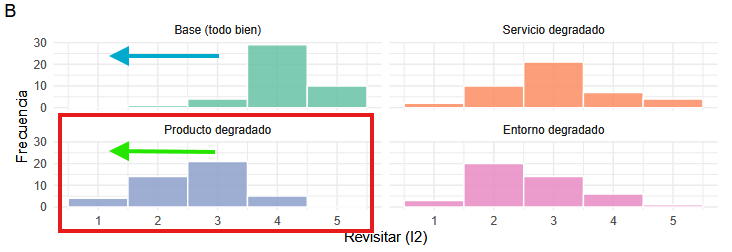
\includegraphics[width=0.7\linewidth]{Revisit_P} 

}

\caption{Impacto de la Manipulación de las variables independientes sobre la Intención de Revisitar del Comensal.}\label{fig:unnamed-chunk-2}
\end{figure}

En la Figura 2 puede comprobarse que, en comparación con la línea de
base, las puntuaciones de los comensales en cuanto a la Intención de
volver al local disminuyen cuando el Producto es degradado,
desplazándose hacia la izquierda (flecha verde).

\begin{figure}[H]

{\centering 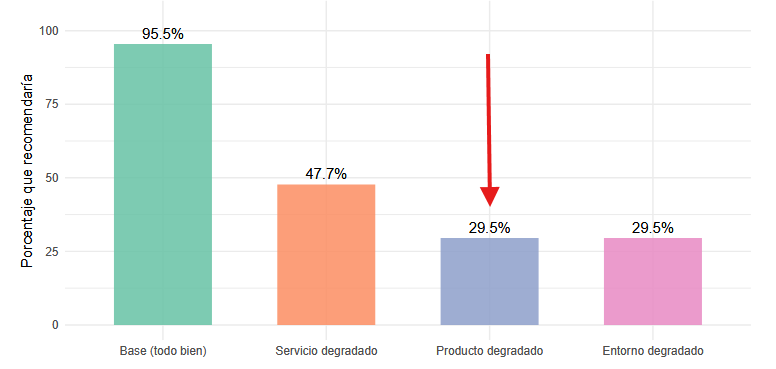
\includegraphics[width=0.7\linewidth]{Rec_P} 

}

\caption{Impacto de la Manipulación de las variables independientes sobre la Intención de Recomendar del Comensal.}\label{fig:unnamed-chunk-3}
\end{figure}

La Figura 3 nos muestra que el impacto de degradar el Producto es, junto
con el de degradar el entorno, el que mayor menoscabo genera en la
intención de recomendar el local por parte del comensal.

A modo de resumen, podemos ver en el cuadro siguiente (Figura 4) la
comparación integral de cómo se comportan todas las variables
independientes. Comprobamos que la variable Producto muestra (según
indica la flecha verde) sus valores más bajos cuando se degrada
experimentalmente tal variable. Esto es una validación indirecta que
corrobora que la manipulación produce el efecto que anticipábamos.

\begin{figure}[H]

{\centering 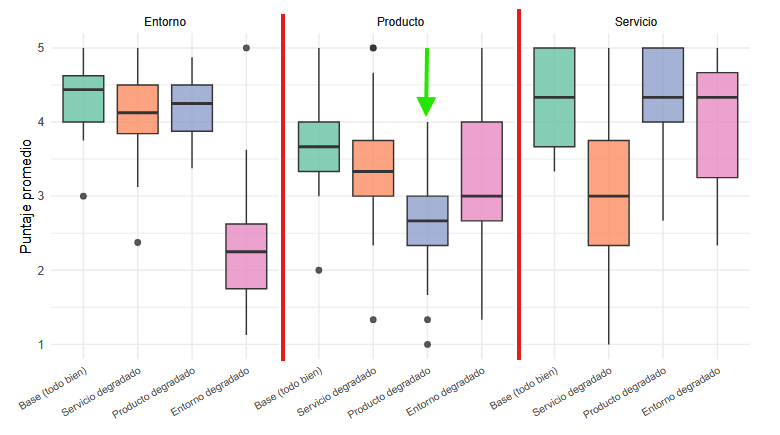
\includegraphics[width=0.7\linewidth]{Comp_P} 

}

\caption{Comparación Integral de las variables independientes según manipulación.}\label{fig:unnamed-chunk-4}
\end{figure}

\subsection{Objetivo Específico: Impacto de la Manipulación del
Servicio}\label{objetivo-especuxedfico-impacto-de-la-manipulaciuxf3n-del-servicio}

\begin{quote}
\emph{Identificar de qué manera los cambios en la calidad del servicio
influyen en la toma de decisiones del comensal.}
\end{quote}

\subsubsection{Impacto de la Manipulación del Servicio sobre la
Satisfacción}\label{impacto-de-la-manipulaciuxf3n-del-servicio-sobre-la-satisfacciuxf3n}

Para detallar los resultados estadísticos del impacto específico de la
manipulación del servicio sobre la Satisfacción del comensal, volvemos a
ver el mismo gráfico indicado en la Figura 1, solo que esta vez hacemos
hincapié en los resultados de la variable Servicio (Figura 5):

\begin{figure}[H]

{\centering 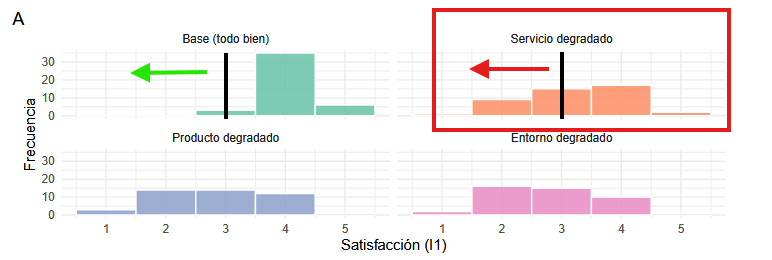
\includegraphics[width=0.7\linewidth]{Sat_S} 

}

\caption{Impacto de la Manipulación de las variables independientes sobre la Satisfacción del Comensal.}\label{fig:unnamed-chunk-5}
\end{figure}

Encontramos que, en efecto, la satisfacción en efecto declina con la
manipulación de la variable, en comparación con la línea base. Este
efecto es estadísticamente fiable (puede verse el detalle numérico en la
tabla resumen en el anexo de contraste de hipótesis).

\end{document}
